\documentclass[12pt,a4paper,spanish]{article}

%package
%\usepackage[T1]{fontenc}
\usepackage[utf8]{inputenc}
\pagestyle{headings}
\usepackage{babel}
\usepackage{xcolor}
\usepackage{amsmath}
\usepackage{amsfonts}
\usepackage{amssymb}
\usepackage[pdftex]{graphicx}
\usepackage[unicode=true] {hyperref}
\usepackage[toc, page, header]{appendix}

\makeatletter

%%%%%%%%%%%%%%%%%%%%%%%%%%%%%% LyX specific LaTeX commands.
\pdfpageheight\paperheight
\pdfpagewidth\paperwidth

%%%%%%%%%%%%%%%%%%%%%%%%%%%%%% User specified LaTeX commands.
\renewcommand{\appendixtocname}{Apendices}
\renewcommand{\appendixpagename}{Apendices}
\newcommand{\rnaemo}{\textbf{\emph{RNAemo}}}

\title{\textbf{RNAemo}\\ \vspace{0.45cm} Especificación de Requerimientos de Software} %ver cual es el paquete de los acentos
\author{Franco Gaspar Riberi}

%\makeatother

\begin{document}
\maketitle\pagebreak{}\tableofcontents{}\pagebreak{}

\newpage

\section{Introducción}
En esta sección se describe un panorama completo del SRS.

\subsection{Propósito}
\par El propósito de este documento es la especificación de requerimientos
de software en el marco de la tesis de grado de la carrera Licenciatura en
Ciencias de la Computación de la UNRC, \textbf{``Estudio de la relación entre divergencia en el uso de codones 
sinónimos entre virus y huésped y presencia de microRNA''}. Internamente este proyecto será denominado \textbf{``}\rnaemo\textbf{''}.
Los requerimientos del software son provistos por integrantes de \textbf{FuDePAN} en su carácter de autores
intelectuales de la solución que se pretende implementar y colaboradores
de dicha tesis.
\par Además, este documento establece la primera etapa de dicha tesis y será utilizado
como parte de la validación final del proyeto.

\subsection{Convenciones del Documento}
Las palabras clave \textbf{DEBE}, \textbf{NO DEBE}, \textbf{REQUERIDO}, \textbf{DEBERÁ}, \textbf{NO DEBERÁ},
 \textbf{DEBERÍA}, \textbf{NO DEBERÍA}, \textbf{RECOMENDADO}, \textbf{PUEDE} y \textbf{OPCIONAL}
en este documento son interpretadas como esta descripto en el documento RFC
2119 [8]. 

\subsection{Audiencia Esperada}
\par A continuación se enumeran las personas involucradas en el desarrollo de la
tesis y que por lo tanto, representan la principal audiencia del presente documento.
\begin{itemize}
	\item \textit{Dr. Roberto Daniel Rabinovich}: Miembro del INBIRS, anteriormente CNRS. Profesor Titular de Virología (Departamento Ciencias Biológicas,
 												CAECE). Colaborador de \textbf{FuDePAN}.
	\item \textit{Lic. Lucía Fazzi}: Licenciada en Genética.
	\item \textit{Maria Pilar Adamo}: Colaborador de tesis, \textbf{FuDePAN}. 
	\item \textit{Daniel Gutson}: Colaborador de tesis, \textbf{FuDePAN}. 
	\item \textit{Lic. Guillermo Biset}: Colaborador de tesis, \textbf{FuDePAN}. 
	\item \textit{Lic. Laura Tardivo}: Directora de tesis, UNRC. 
	\item \textit{Ac. Franco Gaspar Riberi}: Tesista, UNRC.
\end{itemize}

\subsection{Alcance}
\par El producto que se especifica en este documento se denomina \textbf{``Estudio de la relación entre divergencia en el uso de codones 
sinónimos entre virus y huésped y presencia de microRNA''}, y su principal objetivo es contrastar formalmente una idea encomendada y
postulada por el Dr. Roberto Daniel Rabinovich que involucra principalmente 
la molécula de RNA. 

\par Para la comprensión de la hipótesis se deben tener en cuenta algunos hechos referidos al código genético y los microRNA tales como:
\begin{itemize}
	\item El código genético está organizado en tripletes o codones.
	\item El código genético es degenerado\footnote{Implica que al menos uno de los tres nucleótidos (en general el último) puede ser distinto y sin 				embargo codificar para el mismo aminoácido.}: existen más tripletes o codones que aminoácidos, de forma que un determinado aminoácido puede 				estar codificado por más de un triplete. Esos tripletes son conocidos como codones sinónimos. 
	\item En cada especie, se ha seleccionado una proporción de uso de esos codones que guarda relación con la proporción de RNA de transferencia  				correspondiente de manera de optimizar la síntesis proteica.
	\item Para algunos patógenos intracelulares como los virus, existe una divergencia entre el uso de codones sinónimos [20] utilizado por el virus y el 			huésped	correspondiente. El origen de esa divergencia no esta suficientemente esclarecido.
	\item Un microARN [18][19]($_m$$_i$ARN o $_m$$_i$RNA por sus siglas en inglés) es un ARN monocatenario, de una longitud de entre 21 y 25 nucleótidos, 							y que tiene la capacidad de regular la expresión de otros genes mediante diversos procesos, utilizando para ello la ruta de 						ribointerferencia\footnote{También conocido como RNA$_i$ por el acrónico del inglés RNA interference. Corresponde a un mecanismo 							de silenciamiento post-transcripcional de genes específicos, ejercido por moléculas de ARN que, siendo complementarias a un ARN 						mensajero, conducen habitualmente a la degradación de éste.}. Se encuentran codificados en el genoma y juegan un papel importante 							en la regulación de la expresión proteica, en la embriogénesis\footnote{Proceso que se inicia tras la fertilización de los gametos 							para dar lugar al embrión.}, procesos cancerosos e infecciones virales. La generación de los microRNA puede variar según el 						órgano o temporalmente. 
\end{itemize}

\par En este trabajo se estudiará si la divergencia en el uso de codones sinónimos entre virus y huésped contribuye a disminuir la interferencia de los $_m$$_i$RNA en la expresión de los RNA$_m$ de origen viral. De esa manera se contribuirá a comprender mejor la relación virus-huésped y la evolución viral.

\par Dado un conjunto de small-RNA$_s$\footnote{Moléculas de RNA muy pequeñas, dentro de las cuales se encuentra la $_m$$_i$RNA, $_s$$_i$RNA, entre otras.} y una colección de RNA$_m$ de un determinado virus, dado que hay un RNA$_m$ por cada gen, determinar si existen small-RNA$_s$ que se van a hibridar al RNA$_m$. Luego contabilizar la cantidad de small-RNA$_s$ que se hibridarían tanto a la secuencia original como a la secuencia complementaria. De manera similar, realizar el mismo estudio sobre el genoma humanizado\footnote{La humanización refiere al reemplazo de nucleótidos en los tripletes que forman la secuencia de RNA. Se acerca a la proporción de uso de codones utilizado en el humano.} contabilizando la cantidad de small-RNA$_s$ que se hibridan. 
\par Que se hibride o no un small-RNA$_s$ a un determinado RNA$_m$ involucra distintas reglas, siendo la más importante la complementariedad de bases. Pero además existen otras, como la presencia de determinadas bases, proporción de uniones GC y motivos específicos.

\par El proyecto involucrará determinados virus aún no definido. Para tal fin se aplicarán criterios biológicos.

\par El sistema a desarrollar comprenderá las siguientes característica:
\begin{itemize}
	\item Abarcar en su totalidad los requerimientos del problema.
	\item Construir un sistema que puede ser extendido en otros proyectos, brindando un diseño flexible. 
	\item Que proponga un buen uso de las prácticas de diseño para su mejor desempeño.
	\item Que posea abundante documentación clara y precisa.
	\item Lograr un código fuente bien escrito y estructurado respetando las buenas pácticas de programación.
\end{itemize}

\subsection{Descripción general del documento}
\par La estructura de este documento sigue las recomendaciones de la ``Guía para
la especificación de requerimientos de la IEEE'' (IEEE Std 830-1998) [1].
El documento esta organizado en las siguientes secciones generales: 
\par En la \textit{sección 1}, Introducción, se presenta una primera aproximación al proyecto. 
\par En la \textit{sección 2}, Descripción General, se presenta una descripción general de \rnaemo, sus principales
funcionalidades, interfaces y perfiles de usuarios. 
\par En la \textit{sección 3}, Requerimientos, se detallan los requerimientos funcionales específicos de \textbf{\emph{RNAemo}} y
 los principales atributos que \textbf{DEBE} cumplir el software.
\par Por último, se detalla un pequeño apéndice.

\section{Descripción General}
\label{section-desc-gral}
Esta sección describe los requisitos del producto de modo general. Los
requisitos específicos se describen en la sección 3.

\subsection{Perspectiva del Producto}
\par La bioinformática es una disciplina dedicada al análisis de elementos biológicos utilizando a la informática como herramienta principal para generar simulaciones, probar teorías, o realizar cálculos complejos entre otros aspectos. En particular, el producto a desarrollar apunta al cálculo complejo de ciertos datos, los cuales son de gran interés para la biología. El mismo, no será un componente de un sistema de mayor envergadura, sino que por el contrario, será totalmente autónomo e independiente. Además, se espera que sea modular permitiendo:
	\begin{itemize} 
		\item Obtener resultados intermedios y numéricos.
		\item Combinable con otros componentes existentes o a ser desarrollados en el futuro, para obtener nuevos resultados.
	\end{itemize}
\par El sistema se compondrá de los siguiente módulos:
	\begin{itemize}
		\item \textbf{Módulo generador de secuencias humanizadas:} dada una secuencia original, genera una secuencia humanizada. El mismo, corresponde a 																	un componente externo a este desarrollo, y será parte del análisis su obtención.
		\item \textbf{Módulo de matching:} dada una secuencia “larga” de RNA mensajero y una secuencia de small-RNA$_s$, calcular el score de matching a 
											lo largo de todo el genoma del primero. El cálculo se realizará comparando nucleótido a nucleótido de a un
											paso a la vez, determinando cuales hacen matching por complemento. Asimismo, se mostrará con minúsculas 											aquellos nucléotidos que no macheen, en caso contrario, se utilizarán mayúsculas.
		\item \textbf{Módulo maestro (“Master Of Puppets”):} utilizando los módulos anteriores, el presente contabiliza y genera tablas y gráficos leyendo 																una base de datos de small-RNA$_s$. 
	\end{itemize}
	\par Para realizar esta tesis, será necesario contar con datos tanto para realizar las pruebas como para obtener los resultados reales y finales.
	Sin embargo, la obtención de estos datos en volumen está considerado FUERA del ámbito de la Tesis de Licenciatura en Ciencias de la Computación, sí 	sin embargo, se espera recopilar un mínimo de datos para poder hacer las pruebas. Es por esto que se considerará una etapa de búsqueda de
	datos mínimos, dejando el grueso de la búsqueda de datos para \textbf{FuDePAN}. 
	\par El desarrollo de esta tesis seguirá un modelo de cascada, el cual estará compuesto por cuatro iteraciones. 
	\begin{itemize}
		\item \textit{Iteración 1:} corresponde al desarrollo de un software para la generación de tablas comparativas y gráficos. Se hará la búsqueda de 										datos mínimos, y se adaptarán formatos de ser necesarios (bibliotecas de \textbf{FuDePAN} trabajan con el formato 										FASTA). Además se buscará el software existente capaz de humanizar una secuencia dada. Se estudiarán las librerías 										involucradas.
									\par Los datos mínimos incluirán:
									\begin{enumerate}
										\item Un conjunto de al menos 5 RNA mensajeros de virus relevantes.
										\item Un conjunto de al menos 50 small-RNA$_s$ (por ejemplo $_m$$_i$RNA).
									\end{enumerate}
									\par Se espera obtener diferentes tablas comparativas y gráficos que se especifican en las sección 3. 

		\item \textit{Iteración 2:} corresponde a un análisis estadístico sobre las tablas generadas. Se \textbf{DEBE} determinar qué tipo de análisis 										aplicar. Luego, se espera obtener scripts los cuales se ejecutarán y darán como resultado diversos gráficos.

		\item \textit{Iteración 3:} corresponde a un análisis intervirus. Se \textbf{DEBERÁN} tratar diversos virus. Se espera generar resultados considerando más 										de un virus. 

		\item \textit{Iteración 4:} corresponde a la inclusión de folding sobre la estructura secundaria del RNA para el cálculo de matching. Corresponde 										a incluir la estructura secundaria en el módulo de matching. \textbf{DEBERÁ} determinarse si hacer folding, o 										forzarlo y calcular el $\Delta$(G). Asímismo, será necesario estudiar nuevas librerías. 
									Se \textbf{DEBERÁ} ejecutar todo lo mencionado anteriormente para la generación de resultados teniendo en cuenta la  									estructura secundaria.
	\end{itemize}

	\subsubsection{Interfaces del Sistema}
		El producto será capaz de correr al menos en sistemas GNU/Linux, por lo cual sólo se utilizarán librerías compatibles con el mismo.

	\subsubsection{Interfaces de Usuario}		
		En primera instancia, el usuario interactuará con el sistema mediante una CLI, no se proveerá de interfaz gráfica de usuario (GUI).

	\subsubsection{Interfaces de Hardware}
		El producto de software no requerirá hardware específico alguno para su correcto funcionamiento.

	\subsubsection{Interfaces de Software}
		\par Las librerías requeridas para el funcionamiento del sistema son las siguientes:
		\begin{enumerate} 		
			\item \textbf{MiLi:} Colección de pequeñas bibliotecas C++, compuesta unicamente por headers. Sin necesidad de instalación, sin un 									makefile, sin complicaciones. Soluciones simples para problemas sencillos.
						\par \noindent \textcolor{blue}{mili.googlecode.com.}

			\item \textbf{FuD:} Framework para la implementación de aplicaciones distribuidas. 
						\par \noindent \textcolor{blue}{fud.googlecode.com.}

			\item \textbf{BioPP:} Librería de C++ para el manejo de estructuras biológicas, código
						genético, entre otras funciones. 
						\par \noindent \textcolor{blue}{biopp.googlecode.com.}

			\item \textbf{Biopp-filer:} Librería de persistencia para Biopp. 
						\par \noindent \textcolor{blue}{biopp-filer.googlecode.com.} 

			\item \textbf{Odf-gen:} Librería que permite la generación de archivos OpenOffice.
						\par \noindent \textcolor{blue}{odf-gen.googlecode.com.}

			\item \textbf{Fideo:} Provee, entre otras, las funcionalidades necesarias para obtener la energía libre de una secuencia de nucleótidos.
								  Casi la totalidad su código proviene del proyecto \textbf{VAC-O}.
						\par \noindent \textcolor{blue}{vac-o.googlecode.com.}
						\par \noindent \textcolor{blue}{fideo.googlecode.com.}  
		\end{enumerate}

	\subsubsection{Interfaces de Comunicaciones}
		No hay requerimientos especificados.

	\subsubsection{Restricciones de Memoria}	
		\par Este proyecto no presenta restricciones en cuanto a la cantidad de memoria mínima necesaria para operar. El sistema \textbf{DEBERÁ} manejar 			la memoria en forma correcta y sin que ocurran memory leaks. Para realizar depuraciones se utilizará \textit{Valgrind}\footnote{Conjunto de 		herramientas libres que ayuda en la depuración de problemas de memoria y rendimiento de programas. Permite realizar un seguimiento del uso de la 			memoria y detectar problemas. \textcolor{blue}{http://valgrind.org/}}.
		\par Las dependencias externas que serán utilizadas en el producto no deberán ser tenidas en cuenta en el chequeo 
		de memory leaks u otros problemas.
		
	\subsubsection{Operaciones}
		El modo de operación del sistema será: 
		\begin{enumerate}
			\item Invocación por consola por parte del usuario. Esta invocación \textbf{DEBERÁ} tener asociada los siguientes parámetros: 
					\vskip 0.25cm
					\hspace*{0.75cm} • Colección de RNA$_m$. \\
					\hspace*{0.75cm} • Cantidad de random por RNA$_m$. \\
					\hspace*{0.75cm} • Base de datos de small-RNA$_s$. 
			\item Realización de cálculos internos.
			\item En caso de que no se produzcan situaciones erroneas: 
				\begin{itemize}
					\item Exhibición de tablas comparativas de posible hibridación entre microRNA presente en el huésped humano y el RNA presente en la 						  naturaleza y el genoma viral humanizado. 
					\item Exhibición de gráficos con resúmen estadístico a través del cual se podrá inferir, según la tendencia de las curvas, si la 							  divergencia en el uso de codones entre virus-huésped y la presencia de microRNA pueden estar relacionados.
				\end{itemize}
				De lo contrario, el sistema \textbf{DEBERÁ} informar de tal suceso.
		\end{enumerate}

	\subsubsection{Requerimientos de Instalación}
		No se registran requerimientos de instalación.

\subsection{Funciones del Producto}
	\begin{itemize}
		\item \textbf{DEBERÁ} ser capaz de tomar como entrada una colección de RNA$_m$, una cantidad de random por RNA$_m$ y una base de datos de 					small-RNA$_s$. 
		\item \textbf{DEBERÁ} controlar la validez de los parámetros de entrada.
		\item \textbf{DEBERÁ} calcular la secuencia complementaria de la secuencia original de RNA$_m$.
		\item \textbf{BEBERÁ} obtener la secuencia humanizada de la secuencia original de RNA$_m$ utilizando un software externo.
		\item \textbf{DEBERÁ} realizar permutaciones sobre la secuencia de RNA$_m$ conservando la cantidad de cada nucléotido y su tamaño.
		\item \textbf{DEBERÁ} calcular el score de matching, tanto para la secuencia original, como para la secuencia humanizada y la secuencia random.	
		\item \textbf{DEBERÁ} mostrar los resultados al usuario mediante tablas comparativas y gráficos.		
	\end{itemize}

\subsection{Características de Usuario}
	Se identifican un solo tipo de usuario para el sistema:
	\begin{enumerate}
 		\item \textit{Usuario final:} este tipo de usuario refiere a aquellas personas profesionales que utilizarán el 										producto. Sólo deberán interactuar gráficamente (mediante CLI), cargando los datos de entrada 										necesarios y ejecutando el programa para luego obtener el resultado. 
	\end{enumerate}

\subsection{Restricciones}
	El producto \textbf{DEBERÁ} ser desarrollado utilizando el lenguaje de programación C++ [3] y bajo la licencia de software GPLv3 [9]. Además, se 		\textbf{DEBERÁ} respetar los lineamientos generales impuestos por \textbf{FuDePAN} (Thesis Guideline y Coding Guideline). 

\subsection{Trabajo Futuro}
	Inclusión de BLAST como fuente de datos de small-RNA$_s$.

\section{Requerimientos}
\label{section-req} 
En esta sección se detallan específicamente los requerimientos del producto. Se hará hincapié en los requerimientos funcionales de la iteración 1. 	

\subsection{Funciones del Sistema}

	\subsubsection{Interfaces Externas}
		No hay requerimientos especificados.
		
	\subsubsection{Requerimientos Funcionales}
	\begin{itemize}
		\item \textbf{Nombre del requerimiento:} Cargar una collección de RNA$_m$. (RF1).\\
 	    \textbf{Propósito:} Obtener los RNA$_m$ que codifiquen para un mismo virus. Contrala los cuales se determinará si ciertos small-RNA$_s$ 								se hibridan.\\
		\textbf{Input:} Colección de RNA$_m$.\\
		\textbf{Procesamiento:} \\
		\textbf{Output:} \\

		1. \textbf{Sub requerimiento:} Verificar collección de entrada. (RF1.1).\\
 	    \textbf{Propósito:} asegurar que los datos ingresados están dentro de los parámetros aceptables. \\						
		\textbf{Input:} Colección de RNA$_m$.\\
		\textbf{Procesamiento:} \\
		\textbf{Output:} datos válidos o inválidos.\\

		\item \textbf{Nombre del requerimiento:} Cargar una base de datos de small-RNA$_s$. (RF2).\\
 	    \textbf{Propósito:} Obtener los small-RNA$_s$ los cuales serán utilizados para comparar contra los RNA$_m$.\\
		\textbf{Input:} Base de datos small-RNA$_s$.\\
		\textbf{Procesamiento:} \\
		\textbf{Output:} \\

		1. \textbf{Sub requerimiento:} Verificar base de datos de entrada. (RF2.1).\\
 	    \textbf{Propósito:} asegurar que los datos ingresados están dentro de los parámetros aceptables. \\						
		\textbf{Input:} Base de datos small-RNA$_s$.\\
		\textbf{Procesamiento:} \\
		\textbf{Output:} datos válidos o inválidos.\\

		\item \textbf{Nombre del requerimiento:} Especificar la cantidad de secuencias random a generar por RNA$_m$. (RF3).\\
 	    \textbf{Propósito:} refiere a cuantas secuencias random a generar por cada mensajero para realizar controles. Hacer random, significa realizar 								permutaciones al azar sobre la secuencia. \\														
		\textbf{Input:} int.\\
		\textbf{Procesamiento:} \\
		\textbf{Output:} \\

		1. \textbf{Sub requerimiento:} Verificar cantidad de random de entrada. (RF3.1).\\
 	    \textbf{Propósito:} asegurar que el dato ingresado está dentro de los parámetros aceptables. \\						
		\textbf{Input:} int.\\
		\textbf{Procesamiento:} \\
		\textbf{Output:} datos válidos o inválidos.\\

		\item \textbf{Nombre del requerimiento:} Obtener una secuencia humanizada (RF4).\\
 	    \textbf{Propósito:} Obtener una secuencia humanizada para contabilizar los small-RNA$_s$ 
							que se hibridan a ella. Se utilizará un software externo.\\
		\textbf{Input:} secuencia original de RNA$_m$.\\
		\textbf{Procesamiento:} Tomar una secuencia de RNA$_m$, y reemplazar nucleótidos en los tripletes conservando la expresión del aminoácido. Se 									acerca a la proporción de uso de codones utilizado en el humano. \\
		\textbf{Output:} secuencia humanizada.\\

		\item \textbf{Nombre del requerimiento:} Obtener una secuencia random (RF5).\\
 	    \textbf{Propósito:} Obtener una secuencia random para contabilizar los small-RNA$_s$ que se aparean a ella.\\
		\textbf{Input:} secuencia original de RNA$_m$.\\
		\textbf{Procesamiento:} Tomar una secuencia de RNA$_m$, y permutar al azar nucleótidos conservando la misma cantidad de los mismo y el 									mismo tamaño de secuencia. \\
		\textbf{Output:} secuencia random. Por ejemplo, si la secuencia de entrada es \textbf{AATTCCGG}, un permutación válida sería 							\textbf{ATATGCGC}. 	\\

		\item \textbf{Nombre de requerimiento:} Generación de secuencias a partir del RNA$_m$ (RF6).\\
 	    \textbf{Propósito:} Generar una secuencia o segmento por cada posición (de a nucleótidos) del RNA$_m$ en base al apareamiento con respecto a los 								small-RNA$_s$.\\ 
		\textbf{Input:} RNA$_m$, small-RNA$_s$. \\
		\textbf{Procesamiento:} calcular la secuencia complementaria del small-RNA$_s$. Comparar nucleótido a nucleótido comenzando por la posición 1 del 									RNA$_m$, si se corresponden, es decir, si se aparean colocarlo en mayúscula en la secuencia o segmento a generar, de lo 								contrario ponerlo en minúscula. Al llegar al extremo de la secuencia de small-RNA$_s$, avanzar un nucleótido en el
								RNA$_m$.							
		\textbf{Output:} lista de secuencias en la que se puede observar en mayúscula los nucleótidos apareados y en minúscula los no apareados.\\

		1. \textbf{Sub requerimiento:} Determinar apareamiento. (RF6.1).\\
 	    \textbf{Propósito:}  identificar si existe apareamiento entre nucleótidos. \\
		\textbf{Input:} dos nucleótidos. \\
		\textbf{Procesamiento:} comparar los nucleótidos, si son iguales retorna true, de lo contrario false.
		\textbf{Output:} nucleótidos se aperan o no se aparean.\\

		2. \textbf{Sub requerimiento:} Desplazar un lugar en la secuencia. (RF6.2).\\
 	    \textbf{Propósito:} avanzar una posición en la secuencia de entrada. \\
		\textbf{Input:} posición, RNA$_m$. \\
		\textbf{Procesamiento:} recorrer la secuencia de RNA$_m$ hasta llegar a la posición de entrada y retornar desde esa posición la secuencia restante.
		\textbf{Output:} subsecuencia de RNA$_m$. \\

		\item \textbf{Nombre del requerimiento:}  Generación de secuencias a partir del RNA humanizado (RF7).\\
		\textit{Idem} al requerimiento RF6 pero tomando como entrada la secuencia humanizada en lugar de la secuencia original. \\

		\item \textbf{Nombre del requerimiento:} Generación de secuencias a partir del RNA random (RF8).\\
		\textit{Idem} al requerimiento RF6 pero tomando como entrada la secuencia random en lugar de la secuencia original. \\

		\item \textbf{Nombre del requerimiento:} Calcular el score de matching sobre la secuencia original (RF9).\\
 	    \textbf{Propósito:} determinar cuanto matching existe entre el RNA original y el segmento resultante 
							de la hibridación por cada posición del RNA$_m$.\\
		\textbf{Input:} secuencia de RNA original hibrizada. \\
		\textbf{Procesamiento:} Cada hibridación, sea A=T o G=C tendrá un valor representado a través de una dos constantes. Se recorrerá la secuencia 									tomada como entrada y se contará la cantidad de hibridación del tipo A=T por un lado, y por otro lado G=C. Luego se 								calculará el score de matching teniendo en cuenta las constantes. 								
		\textbf{Output:} score de matching.\\

		\item \textbf{Nombre del requerimiento:} Calcular el score de matching sobre la secuencia humanizada (RF10).\\
		\textit{Idem} al requerimiento RF9 pero tomando como entrada la secuencia de RNA humanizada hibrizada. \\
		
		\item \textbf{Nombre del requerimiento:} Calcular el score de matching sobre la secuencia random (RF11).\\
		\textit{Idem} al requerimiento RF9 pero tomando como entrada la secuencia de RNA random hibrizada. \\

		\item \textbf{Nombre del requerimiento:} Construir tablas comparativas (RF12).\\
 	    \textbf{Propósito:} Exibir los datos anteriormente mencionados en forma de tabla para una mejor comparación y permitiendo así llegar a 								ciertas conclusiones. Se construiran tantas tablas como combinación de RNA$_m$ y small-RNA$_s$ existan.\\
		\textbf{Input:} posición, RNA$_m$, RNA humanizado, RNA random, score matching original, score matching humanizado y score matching random.\\
		\textbf{Procesamiento:} . Insertar cada dato de entrada en una columna diferente de la tabla.\\
		\textbf{Output:} Las tablas a generar se pueden observar en la Figura~\ref{table}.
			\vskip 0.5cm
			\begin{figure}[h]
				\begin{center}
					\includegraphics[width=6.2638in,height=1.3744in]{table2.png}
					\caption{Estructura de las tablas a generar.}
					\label{table}
				\end{center}
			\end{figure}
		
		\vskip 10 cm
		\item \textbf{Nombre del requerimiento:} Generar gráficos (RF13).\\
 	    \textbf{Propósito:} Exhibir la información a través de gráficos para una comprensión más clara.\\
		\textbf{Input:} posición, RNA$_m$, RNA humanizado, RNA random, score matching original, score matching humanizado y score matching random..\\
		\textbf{Procesamiento:} .\\
		\textbf{Output:} Las gráficos a generar se pueden observar en la Figura~\ref{graphic}.
			\begin{figure}[h]
				\begin{center}
					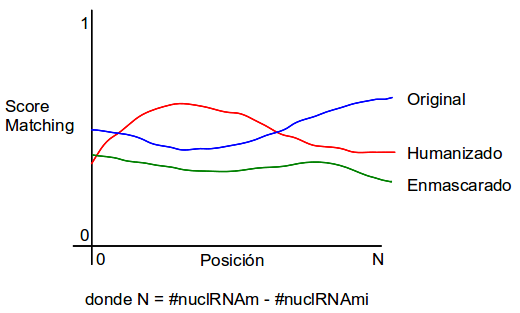
\includegraphics[width=4.8638in,height=2.8744in]{graphics.png}
					\caption{Estructura de los gráficos a generar.}
					\label{graphic}
				\end{center}
			\end{figure}

%requerimientos no funcionales
\subsection{Restricciones de Rendimiento}
No hay requerimientos especificados.

\subsection{Herramientas}
	Se utilizará \textit{fudepan-build} [15] como build system.

\subsection{Base de Datos}
	\par El sistema requerirá de una base de datos de small-RNA$_s$. En caso alternativo, se permitirá el uso de BLAST para generar secuencias. 

\subsection{Restricciones de Diseño}
\par El producto \textbf{DEBERÁ} cumplir con los siguientes principios de diseño de la
programación orientada a objetos. Los 5 primeros, son también conocidos por
el acrónimo \textbf{``SOLID''} [2].
\begin{itemize}
	\item \textbf{S}ingle responsibility principle (SRP)
	\item \textbf{O}pen/closed principle (OCP)
	\item \textbf{L}iskov substitution principle (LSP)
	\item \textbf{I}nterface segregation principle (ISP)
	\item \textbf{D}ependency inversion principle (DIP)	
	\item Law of Demeter (LoD)
\end{itemize}

\subsection{Atributos del Software}
\par El código del producto \textbf{DEBERÁ}:
\begin{itemize}
 \item Compilar sin advertencias, o las advertencias aceptadas \textbf{DEBERÁN} estar documentadas.
 \item Cumplir con el estándar ANSI C++ y el ``\textit{Coding Guideline}'' definido por \textbf{FuDePAN}.
\end{itemize}
\par El software \textbf{DEBERÁ}:
\begin{itemize}
	\item Funcionar sin memory leaks según \textit{Valgrind}.
	\item Tener al menos un 85\% de cobertura con pruebas automatizadas.
\end{itemize}

\pagebreak

\begin{appendices} 
  \section{Definiciones, Acrónicos y Abreviaturas}
\label{appendix-acro}
\begin{itemize}
	\item \textbf{RNAemo:} Nombre que recibe el presente producto.
	\item \textbf{UNRC:} Universidad Nacional de Río Cuarto.
	\item \textbf{FuDePAN:} Fundación para el Desarrollo de la Programación en Ácidos Nucleicos [17].
	\item \textbf{INBIRS:} Instituto Biomédico en Retrovirus y SIDA.
	\item \textbf{CNRS:} Centro Nacional de Referencia para el SIDA.
	\item \textbf{SIDA:} acrónimo de síndrome de inmunodeficiencia adquirida. También abreviada como VIH-sida o VIH/sida.
	\item \textbf{CAECE:} Centro de Altos Estudios en Ciencias Exactas.
	\item \textbf{IEEE:} Institute of Electrical and Electronics Engineers.
	\item \textbf{SOLID:} acrónimo nemotécnico introducido por Robert C. Martin en la
							década de 2000, que representa cinco principios básicos de programación
							y diseño orientado a objetos
	\item \textbf{GPL:} \textit{G}eneral \textit{P}ublic \textit{L}icense.	
	\item \textbf{SRS:} Especificación de requerimientos.
	\item \textbf{FuD:} FuDePAN Ubiquitous Distribution [14]. Framework para el desarrollo de aplicaciones distribuídas a través de disposiciones 							heterogéneas y dinámicas de nodos de procesamientos.
	\item \textbf{CLI:} Interfaz de Línea de Comandos, por su acrónimo en inglés de Command Line Interface. Permite dar instrucciones a algún programa 							informático por medio de una línea de texto.
	\item \textbf{FASTA:} es un formato de archivos informáticos basado en texto, utilizado para representar secuencias de ácidos nucleicos, y en el que 							  los pares de bases o los aminoácidos se representan usando códigos de una única letra. El formato también permite incluir nombres 						  de secuencias y comentarios que preceden a las secuencias en sí.
	\item \textbf{Nucleótido:} molécula orgánica formada por la unión covalente de un monosacárido de cinco carbonos (pentosa), una base nitrogenada y un 								   grupo fosfato.
	\item \textbf{Tripletes:} conjunto de tres nucleótidos que determinan un aminoácido concreto, también conocido como codón.

	\item \textbf{Aminoácido:} molécula orgánica que conforma la proteína.
	\item \textbf{RNA:} Ácido ribonucléico. Es un tipo de ácido nucleico compuesta por nucléotidos esencial para la vida.
	\item \textbf{DNA:} Ácido desoxirribonucleíco. Es un tipo de ácido nucleico, forma parte de todas las células.
	\item \textbf{RNA$_m$:} RNA mensajero. Se encuentra tanto en el núcleo como en el citoplasma celular. Su función es portar el código genético para
							las proteínas, es decir, transportan las instrucciones de codificación de las proteínas desde el DNA.
	\item \textbf{$_s$$_i$RNA:} short interfering RNA. Corresponde a una clase de RNA de cadena doble presente en células eucariotas.
	\item \textbf{$_m$$_i$RNA o microRNA:} Corresponde a una clase de RNA de cadena simple presente en células eucariotas. 
	\item \textbf{small-RNA$_s$:} Moléculas muy pequeñas de RNA. Dentro de la clasificación de RNA, aparecen como RNA no codificante.
	\item \textbf{Proteína:} macromolécula formada por cadenas lineales de aminoácidos. Se considera proteína a aquellas cadenas de aminoácidos  enlazados 								cuyo peso molecular es superior 6000 Daltons.
	\item \textbf{Virus:} Entidad biológica que para reproducirse necesita de una célula huésped.	
%	\item \textbf{Virus de la Polio:} virus que sólo infecta a los humanos. Afecta el sistema nervioso central, más específicamente, la sustancia gris en 										la médula y tronco del encéfalo.  
	\item \textbf{$\Delta$(G) o energía libre:} Es el potencial químico que se minimiza cuando un sistema alcanza el equilibrio a presión y 								temperatura constante. [13] 
%	\item \textbf{Proceso de melitación:}	
%	\item \textbf{Silenciamiento genético transcripcional:}	
%	\item \textbf{RNA codificante:} es aquel RNA que genera proteínas. Se encuentra el RNA$_m$.
	\item \textbf{RNA no codificante:} es aquel RNA que no genera proteínas. Se encuentra el RNA transcripcional y small-RNA$_s$.
	\item \textbf{Humanización-Deshumanización:} refiere a mutar de forma silente una secuencia. Esto significa, mutar nucleótidos de un triplete 													conservando la expresión del aminoácido. La diferencia entre humanización y deshumanización radica en que 													si los tripletes por los que se muta son o no los preferenciales.				
	\item \textbf{Mutación silente:} Las mutaciones silentes ocurren cuando se produce un cambio de un sólo nucleótido de DNA dentro de una porción de un 										gen codificador para una proteína que no afecta la secuencia de aminoácidos que componen la proteína para el gen. Un 										cambio en un nucleótido, sin embargo, no siempre cambia el significado de un triplete. El triplete mutado puede aún 									representar el mismo aminoácido. Y cuando los aminoácidos de una proteína siguen siendo los mismos, esta mantiene su 										estructura y función.				
	\item \textbf{BLAST:} \textit{B}asic \textit{L}ocal \textit{A}lignment \textit{S}earch \textit{T}ool [16]. Es un programa de alineamiento de 										secuencias, ya se de DNA, RNA o proteínas. Es capaz de comparar una secuencia problema (denominada query) contra una 										gran cantidad de secuencias almacenadas en una base de datos. Encuentra las secuencias de la base de datos que tienen 										mayor parecido a la secuencia query. BLAST es desarrollado por los Institutos Nacionales de Salud del gobierno de 										Estados Unidos.
	\item \textbf{Codones sinónimos}: término más conocido como \textit{``codon usage bias''}. Refiere a la diferencia en la frecuencia de ocurrencias de 										  codones en la codificación del DNA.


%	\item \textbf{Distancia de hamming:} se denomina distancia de Hamming a la efectividad de los códigos de bloque y depende de la diferencia entre una 											palabra de código válida y otra. Cuanto mayor sea esta diferencia, menor es la posibilidad de que un código válido 											se transforme en otro código válido por una serie de errores. A esta diferencia se le llama distancia de Hamming, y 										se define como el número de bits que tienen que cambiarse para transformar una palabra de código válida en otra 										palabra de código válida.
\end{itemize}
	
  \section{Manejo de inputs}
	\label{appendix-def}
\par Para la manipulación de los datos se usaran cadenas de caracteres que representan tanto cadenas de DNA como cadenas de RNA para representar genes como nucleóticos.
\begin{itemize}
	\item \textbf{nuc\_arn} $\to$  a $\vert$ u $\vert$ c $\vert$ g $\vert$ \_ 
	\item \textbf{gen\_arn} $\to$ (\textbf{nuc\_arn})\textsuperscript{+}

	\item {nuc\_adn} $\to$ a $\vert$ t $\vert$ c $\vert$ g $\vert$ \_
	\item {gen\_adn} $\to$ (\textbf{nuc\_adn})\textsuperscript{+}
\end{itemize}
\par Para formar cadenas más complejas, tales como aminoácido y proteínas, se usará:
\begin{itemize}
 	\item \textbf{aminoacido} $\to$ Ala $\vert$ Arg $\vert$ Asn $\vert$ ...	
	\item \textbf{proteina} $\to$ \textbf{aminoacido}(\textbf{aminoacido})\textsuperscript{+}
\end{itemize}

  \section{Sugerencias}
\label{appendix-formulates}

	\large \textbf{C.1 Pseudo-Código para enmascarar nucleótidos (``M'')}
	\par Para determinar que nucleótidos deben ser reemplazados por una ``M'' en la generación de secuencias enmascaradas, 		se propone el siguiente Pseudo-Código.

    \begin{verbatim}
        input: nuc_mensajero, nuc_mirna

        if (nuc_mensajero == complemento(nuc_mirna)) {
            if (nuc_mensajero.apareado()){
                print "M"
            }else{
                print upper_case(nuc_mirna)			
            }	
        }else{
                print lower_case(nuc_mirna)
        }                
    \end{verbatim}

	\large \textbf{C.2 Scores matching}
	\par Para calcular el score de matching sobre las secuencias (secuencia original, secuencia humanizada) se sugiere la 		fórmula (\ref{eq}).

	\begin{equation}	
		\label{eq} \frac{(\#AT \times constAT + \#GC \times constGC)}{(totalAT \times constAT + totalGC \times constGC}
	\end{equation}	

	\par donde:
		\begin{itemize}
			\item \textbf{\#AT:} cantidad de Adenina que hace matching con Timina, o viceversa.
			\item \textbf{\#GC:} cantidad de Guanina que hace matching con Citosina, o viceversa.
			\item \textbf{constAT:} valor predeterminado para el apareo A=T.
			\item \textbf{constGC:} análogo al anterior, pero con apareo G=C.
			\item \textbf{total AT:} total de adedina y timina (apareadas o no).
			\item \textbf{totalGC:} total de guanina y citosina (apareadas o no).	
		\end{itemize} 

	\par Esta fórmula permitirá calcular dos score, uno de ellos empleando constantes \textbf{constAT} y \textbf{constGC} 		de valor 1 (cuyo resultado corresponderá a un porcentaje), y para el otro se emplearan constantes de folding.
 

  \section{Referencias}
\label{appendix-ref}
[1] IEEE Recommended Practice for Software Requirements Specifications. Copyright © 1998 by the Institute of Electrical and Electronics Engineers, Inc. All rights reserved. Published 1998. Printed in the United States of America. ISBN 0-7381-0332-2. \\

[2] SOLID: ``Design Principles and Design Patterns'', Robert C. Martin. \textcolor{blue}{http://www.objectmentor.com/resources/articles/Principles\_and\_Patterns.pdf} \\

[3] C++: Lenguaje de programación. \textcolor{blue}{http://www.cplusplus.com} \\

[4] G. Biset, D. Gutson, and M. Arroyo, “A framework for small distributed projects and a protein clusterer application”, 2009. \\

[5] G. Biset, D. Gutson, and M. Arroyo, “Fud: Design and implementation of a framework for small distributed applications”, 2009. \\

[6] B. Meyer, “Object-Oriented Software Construction”, Second Edition, Santa Barbara: Prentice Hall Professional Technical Reference, 1997. \\

[7] G. Booch, J. Rumbaugh, and I. Jacobson, “Unified Modeling Language User Guide”, Second Edition, 2005. \\

[8] RFC 2119. \textcolor{blue}{http://tools.ietf.org/html/rfc2119} \\

[9] GNU General Public License. \textcolor{blue}{http://www.gnu.org/licenses/} \\

[10] H. Curtis, N. Sue Barnes, A. Schnek and G. Flores, “Biología”, Editorial Médica Panamericana S.A, 2006, ISBN: 950-06-0423-X. \\

[11] B. Pierce, “Genética. Un enfoque conceptual”, Tercera Edición, Editorial médica panamericana S.A, ISBN: 978-84-9835-216-0. \\

[12] A. Blanco, “Química Biológica”, Séptima Edición, Editorial El Ateneo. \\

[13] $\Delta$(G): \textcolor{blue}{http://en.wikipedia.org/wiki/Gibbs\_free\_energy} \\

[14] FuD : \textcolor{blue}{http://code.google.com/p/fud/} \\

[15] fudepan-build: \textcolor{blue}{http://fudepan-build.googlecode.com} \\

[16] BLAST: \textcolor{blue}{http://blast.ncbi.nlm.nih.gov/Blast.cgi} \\

[17] FuDePAN: \textcolor{blue}{http://www.fudepan.org.ar/} \\

[18] Vinay S. Mahajan, Adam Drake and Jianzhu Chen, “Virus-specific host miRNAs: antiviral defenses or promoters of persistent infection?”. \\

[19] Man Lung YEUNG, Yamina BENNASSER, Shu Yun LE and Kuan Teh JEANG, “siRNA, miRNA and HIV: promises and challenges”. \\

[20] Gareth M. Jenkins and Edward C. Holmes, “The extent of codon usage bias in human RNA viruses and its evolutionary origin”, 2003. \\

[21] Comeron JM and Aguadé M. “An evaluation of measures of synonymous codon usage bias”, 1998. \\

[22] Haruhiko Siomi and Mikiko C. Siomi, “On the road to reading the RNA-interference code”. \\
     
\end{appendices}

\end{document}

\end{document}
